%!TEX root = foo-thesis.tex

\chapter{Introduction to Global Illumination and Previous Work}
\label{chap:introductionGI}

This chapter starts by giving a rough overview of lighting in computer graphics and locate and distinguish global illumination in this vast research field.
Subsequently, it lays the groundwork for the following chapters by introducing the conceptual and theoretical foundations of global illumination in general and many-light methods in particular, combined with an overview of the related work in those topics.


\section{A High-Level Overview of Lighting in Computer Graphics}

Before examining the different lighting effects simulated in computer graphics, it is worth pointing out that real-world physics do not know most of the distinctions made later in this section. Many effects and phenomena in lighting can be reduced to a basic set of interactions of photons, which are emitted by light sources and then reflected, refracted or absorbed by matter.

In practice, simulating individual photons and atoms is obviously infeasible and unnecessary to simulate for most computer graphics applications. Instead, computer graphics researchers have examined the different real-world light phenomena and simulated them separately, using different approaches and approximations for each of them to stay within their respective performance budget.


The following gives a rough (and non-comprehensive) overview over these lighting effects and locate global illumination within them. Our most top-level distinction is between the interaction of light with the scene's surfaces, and the transport of light through empty space in the scene.

\paragraph{Light-Surface Interaction.}

To determine how much and in what direction incoming light is reflected from surfaces, \textit{bi-directional reflectance distribution functions} (BRDFs) are used. While the recent shift to physically-based BRDFs has brought more unified models to real-time computer graphics, several materials such as transparent (e.\,g.\ glass) or highly translucent ones (e.\,g.\ skin) are still handled separately.


\paragraph{Light Transport.}

In order for light to interact with surfaces, it needs to be ``transported'' to them from light sources. The simplest case, light that hits only one surface before reaching the camera, is called \textbf{direct light}. To determine surfaces that are directly lit by a certain light source, shadow maps are commonly used in real-time computer graphics.

Direct light usually has a single point as origin in the case of point lights, or consists of entirely parallel light rays in the case of directional lights. This structuredness makes it comparatively easy to compute.

\textbf{Indirect light} on the other hand is bounced off at least two surfaces before reaching the camera. Since each point that is directly lit now reflects light into arbitrary directions, this process is much less structured and thus harder to compute. To cope with this complexity, indirect light has been separated into small-scale and large-scale indirect light. An intermediate step for medium-scale indirect lighting has also been proposed \citep{reed:2012:mediumAO}.

The simulation of \textbf{small-scale indirect light} has been made popular with \textit{screen-space ambient occlusion} (SSAO, \cite{Mittring:2007:Cryengine2}). While this should be more accurately described as small-scale indirect \textit{occlusion}, since it only darkens occluded areas, \textit{screen-space directional occlusion} (SSDO, \cite{Ritschel:2009:SSDO}) actually performs a form of indirect lighting, albeit a limited one. \citet{jimenez:2016:AO} have finally put this technique onto a physically based foundation.

Small-scale indirect lighting techniques such as SSAO are important for accentuating small geometric details in objects and providing a sort of contact shadow as a visual cue for the proximity of objects to each other.

In contrast, \textbf{large scale indirect lighting} provides more realistic lighting for entire scenes. While it has been simulated in real-time for static scenes for a while, large-scale indirect lighting for fully dynamic scenes has yet to reach mainstream in real-time applications. More on this in the next section.
\\
\\
The term \textit{global illumination} (GI) has been used for varying sets of lighting effects throughout the literature. In this thesis, it is used to describe the lastly discussed aspect, large-scale indirect lighting.



\section{Introduction to Global Illumination}

This section introduces global illumination by outlining its advantages and describing its theoretical foundations. Thereafter it prepares for the following section on related work by giving an overview of techniques used previously to simulate (non-dynamic) global illumination, and structures the process of computing global illumination by identifying individual building blocks.

For another comprehensive introduction to global illumination, see \citet{Ritschel:2012:GISTAR}.

\subsection{Motivation}
The single overarching advantage of simulating global illumination in graphics applications is the added realism which leads to a host of benefits. An obvious one is the greater immersion achieved in movies and video games, but also architectural and e-commerce visualization applications can provide better assistance to its users through more realistic renderings. For instance, in architectural visualization, the colors of the furniture, carpets etc.\ are influencing the overall tone of the scene, e.\,g.\ by coloring the walls slightly, leading to a better basis for real-world design decisions.

Real-time techniques that allow camera movements in a given scene and lighting setup on the one hand enable simulation of GI in applications that are inherently real-time, e.\,g.\ video games.

On the other hand, even applications that do not require real-time frame rates can benefit from such techniques. For instance, while the features that are covered in this thesis are basically solved for offline rendering, the film industry can benefit from real-time GI techniques during production through faster testing of e.\,g.\ different camera angles. Archvis applications can satisfy more use cases by implementing interactive walkthroughs.

Allowing changing geometry provides additional benefits: Games can create new experiences with changing level geometry e.\,g.\ through destruction, level designers and lighting artists can expect a more natural workflow without having to resort to workarounds like fake lights, artists in filmmaking benefit from shorter iteration cycles, and visualization tools provide immediate feedback to changes in e.\,g.\ interior decoration in the case of archvis.


\subsection{Theory}
\label{sec:intro:gi:theory}


% based on https://github.com/naps62/msc-thesis/tree/ee10a36eecbb691ba1a67b4c5367967023d07440/doc/common/equations
\newcommand{\dir}{\vec\omega} % directions are represented by greek omega character

\newcommand{\outgoingDir}{ \dir_o}
\newcommand{\incidenceDir}{\dir_i}

\newcommand{\outgoingRadiance}{  L_o(x, \outgoingDir)}
\newcommand{\emittedRadiance}{   L_e(x, \outgoingDir)}
\newcommand{\reflectedRadiance}{ L_r(x, \outgoingDir)}
\newcommand{\incidentRadiance}{  L_i(x, \incidenceDir)}

\newcommand{\brdf}{f_r} % brdf function name

\newcommand{\surfaceNormal}{\vec{n}}

This section will explain the significance of global illumination using the rendering equation \citep{Kajiya:1986:RenderingEquation}. The most basic form of the rendering equation is as follows:

% \begin{figure}[!htp]
  \begin{equation}
    \outgoingRadiance = \emittedRadiance + \reflectedRadiance
  \label{eq:renderBasic}
  \end{equation}
% \end{figure}
\noindent
This describes the outgoing radiance $L_o$ from a surface point $x$ in the direction $\outgoingDir$, which is equal to the emitted radiance $L_e$ plus the reflected radiance $L_r$.

The reflected radiance can be defined as

% \begin{figure}[!htp]
  \begin{equation}
    \reflectedRadiance = \int\limits_{\Omega} \brdf(x, \incidenceDir, \outgoingDir)\incidentRadiance (\incidenceDir \cdot \surfaceNormal) d \omega_i
  \label{eq:render}
  \end{equation}
% \end{figure}
\noindent
where $\Omega$ is the upper hemisphere of point $x$, $\brdf$ is the BRDF of the surface, $L_i$ the incident radiance and $\surfaceNormal$ the surface normal at point $x$.

While this is the most common representation of the rendering equation, \citet{Kajiya:1986:RenderingEquation} defined the reflected radiance using an integral over all surface points, not all directions:

% \begin{figure}[!h]
  \begin{equation}
    \reflectedRadiance = \int\limits_{S} \brdf(x, \incidenceDir, \outgoingDir) \incidentRadiance (\incidenceDir \cdot \surfaceNormal) V(x, x') d x'
  \label{eq:renderWithVisibility}
  \end{equation}
% \end{figure}
\noindent
where $\incidenceDir$ is now defined as the normalized difference vector between $x$ and $x'$ and $S$ is the (infinite) set of all surface points. Since not all surface points are visible from $x$, a visibility term $V$ has been added that is $1$ if $x$ and $x'$ are mutually visible, $0$ otherwise.

This equation illustrates a major difficulty when simulating global illumination, namely the integral that needs to be solved for the infinite set of surface points. To approximate this integral, one generally picks a random set of points or clusters points to form surface patches. Even then, the performance requirements are generally too high for real-time computer graphics. As a result, this integral is either solved in a preprocessing step for static parts of the scene, or solved only for the set of points that are considered light sources, discarding a large portion of the light energy in the scene and heavily altering the rendered output. In fact, area lights are often ignored or approximated because they again would require solving this integral for an infinite number of points.

Another difficulty made explicit by \Cref{eq:renderWithVisibility} is the visibility term. Even with an algorithm that transfers light between points or surface patches at a sufficient resolution and sufficient speed, the visibility term requires the addition of another algorithm that tests for each pair of surface elements whether any other surface element is located between them. This is often one of the most computationally intensive parts of global illumination algorithms.



\subsection{The Path to Real-Time Dynamic Global Illumination}

Originally, global illumination has been ignored in 3D computer graphics, especially in interactive applications. To avoid completely unlit areas, an ambient term has been used that uniformly adds light to all surfaces.

For large-scale indirect lighting, light maps have seen widespread use since they have been introduced in the video game Quake \citep{Abrash:1997:BlackBook}. This technique is inherently static since the texturing of scene surfaces is an offline preprocessing step, and it is inherently large-scale since large texels are used to avoid excessive memory requirements.

Games have used variations of \emph{precomputed radiance transfer} (PRT, \cite{sloan:2002:PRT}) to accommodate for changing lighting conditions. For instance, \citet{stefanov:2012:PRTinFarCry3} uses probes instead of the scene geometry to store the PRT results to be able to light dynamic objects. However, even though dynamic objects receive indirect lighting, they are unable to affect indirect lighting of other objects, a commonly made compromise.

Besides not fully supporting dynamic objects, the long precomputation times of conventional global illumination methods are a common hindrance in the workflow of artists. Real-time dynamic global illumination, being the solution to both of these problems, has yet to reach widespread use in real-time applications due to the high performance requirements.


\subsection{Components of Real-Time Dynamic Global Illumination}
\label{sec:intro:gi:components}

Before the next section dives into the current research around real-time dynamic GI, this section will structure the different components that most methods consist of.

Generally speaking, real-time GI consists of three steps:

\paragraph{Direct lighting or light injection.}
Since the light sources can be very (if not infinitely) small and can be unwieldy to work with for some techniques, the first step of the light propagation, sometimes called ``light injection'', can be separated and used to compute areas that are directly lit by the scene lights. These areas are then used as starting point for the GI algorithm. Other techniques use this method purely as an optimization, since the first light bounce can be easier to compute than subsequent bounces.

\paragraph{Light propagation.}
Starting from the light source or directly lit surfaces, this step sends out the light and records where it hits scene geometry. This might be done repeatedly to simulate multiple light bounces.

\paragraph{Final gathering.}
Several techniques perform one last step that, instead of propagating light from lit surfaces into all directions, gathers light from lit surfaces into areas that are visible to the camera (more specifically, into \textit{receiving elements}, see below for further explanation). This is a common optimization that guarantees that the calculations are relevant to the currently rendered frame, whereas the light propagation step is often more unguided and oblivious to the current viewport.
\\
\\
Note that not all techniques implement all of these steps. For instance, performing direct lighting and a final gathering step while omitting the light propagation step is enough for simulating one indirect bounce. Brute-force ray-tracing can be done with step 2 alone, and light propagation volumes (see next section) omit the final gathering step.
\\
\\
There are two more essential components, or rather, design decisions to be made:

\paragraph{Visibility testing.}
To prevent light from incorrectly shining through objects or walls, the visibility term in \Cref{eq:renderWithVisibility} needs to be solved. Since brute-force ray casting is prohibitively slow, this needs special acceleration structures or alternative approximations, like replacing ray casts with (a moderate amount of) shadow maps. As mentioned previously, this part uses a substantial if not most of the computation time for many of the global illumination approaches presented in the next section.

\paragraph{Choice of receiving elements.}
The final gathering step gathers light into areas that are visible to the camera. These areas can be represented by several forms of \textit{receiving elements}. Besides directly using pixels in screen-space, other choices are texels in texture-space, surfels or voxels in world- or view-space or other virtual objects placed in the scene, e.\,g.\ in the form of spherical harmonics, which are then interpolated between to shade the individual pixels.

Technically, the light propagation step also necessarily uses some form of receiving elements (which might differ from the ones that are used during final gathering), but we use the term for those data structures that are used to perform the actual per-pixel shading.
\\
\\
As with most lighting concepts, real-time GI is often additionally separated into a diffuse and specular component, since the diffuse part is both easier to plausibly simulate because of its low-frequency nature, and it is more important for the visual quality compared to the specular part. For the same reasons, we only cover the diffuse part in this thesis.



\section{Previous Work on Real-Time Dynamic Global Illumination}

This section presents previous work on global illumination while focusing on methods that work in real-time and support dynamic scenes, excluding many-light methods which are covered separately in the next section.

For a more comprehensive study of interactive global illumination methods, refer to \citet{Ritschel:2012:GISTAR}.

\subsection{Point-Based Approaches}

Based on the work of \citet{Bunnell:2005:AO}, point-based global illumination has been used for offline rendering in the film industry \citep{christensen2008point}.
Despite its name, the geometry representation used to approximate the scene geometry consists of disk-shaped surface elements (\emph{surfels}).
These surfels are then organized into the leaves of a tree structure, while the higher-level nodes are aggregate representations of all nodes they contain.
This tree is then used to compute visibility and propagate light between the surfels.
While \citet{Bunnell:2005:AO} uses a rough approximation for computing visibility, \citet{christensen2008point} uses ray tracing or spherical harmonics based on the distance between surfels to compute an accurate simulation of global illumination.
\citet{Ritschel:2009:microrendering} achieve interactive frame rates by using the GPU to perform the final gathering step, which renders the scene into a \emph{micro-buffer} for each receiving element (in their case, screen-space pixels).
Due to the large amounts of surfels required and the necessary tree structure, this technique is best suited for static or very small scenes.



\subsection{Light Propagation Volumes}

Originally proposed by \citet{Kaplanyan:2010:LPV} and extended by \citet{Kaplanyan:2010:LPV2}, this technique reduces the scene's geometry to two voxel grids, called \emph{light propagation volume} (LPV) and \emph{geometry volume} (GV) respectively. It then then injects light from primary light sources into the LPV, and inserts the scene geometry into the GV. Starting from there, the light is iteratively propagated from each illuminated voxel to its neighboring voxels until it is determined through the GV that the path is occluded. However, since inaccuracies of the propagation process accumulate over the iterations, this approach is inaccurate when dealing with long distances between sender and receiver.


\subsection{Voxel Cone Tracing}

Similar to light propagation volumes, the scene is first reduced to voxels and light from primary sources is injected. However, instead of propagating the light through the grid, the light is collected starting at receiving elements, usually pixels in screen-space, by tracing cones through the grid.
While the original proposal \citep{Crassin:2012:OctreeVCT} uses a sparse voxel octree to represent the scene, \citet{Panteleev:2015:VXGI} introduces clip-maps that use several levels of equally-sized voxel grids to represent the scene with varying resolution depending on the distance to the camera.
Both approaches can simulate specular reflections for moderately glossy surfaces. While the voxel octree is expensive to update with dynamic objects, the clip-maps are faster in this regard, but still need relatively large amounts of VRAM for higher quality levels. Lower quality levels exhibit noticeable voxelization artifacts.


\subsection{Ray-Tracing}

Several attempts have been made to adapt ray-tracing to be usable in a real-time context.
\citet{Thiedemann:2011:VGI} trace rays through a voxel grid, but have to limit the ray's maximum distance for performance reasons and, similar to voxel cone tracing, suffer from high memory requirements.
\citet{Tokuyoshi:2012:pathtracingrasterization} trace rays using rasterization, but at the cost of a severe performance impact since they render the whole scene multiple times.
\citet{Chen:2016:Compactvoxels} use one bit per voxel to indicate whether it is opaque or not, and look up lighting information directly in an RSM during the final gather phase. They too achieve only interactive frame rates.


\subsection{Radiance Caching}

Partly orthogonal to the previous sections, radiance caches are a different form of receiving elements that are placed in world- or screen-space and capture the incoming radiance. During actual shading, the nearest caches are interpolated. The major advantage is the reduction of the number of receiving elements for which incoming light needs to be gathered.
The original proposal cached irradiance values \citep{Ward:1988:IrradianceCaching}. The resulting loss of detail during interpolation and inability to compute specular reflections was overcome by radiance caching \citep{Krivanek:2005:RadianceCaching} at a performance loss. \citet{Scherzer:2012:PreconvolvedRadianceCaching} achieved real-time frame rates for static geometry and another improvement in efficiency was proposed by \citet{Rehfeld:2014:ClusteredPreconvolvedRadianceCaching}.
Radiance caching is orthogonal to the other techniques in so far as visibility still needs to be solved by other means, and using it introduces new problems such as temporal stability of the cache placement.


\subsection{Screen-Space Approaches}

Screen-space approaches inherently suffer from the lack of information about objects that are outside of the view frustum or occluded. The latter is alleviated by deep g-buffers \citep{Mara:2014:DeepGBuffers, Mara:2016:DeepGBuffers2}, but working only within the frustum, even this approach is limited to small to medium-scale indirect illumination.



\section{Introduction to Many-Light Methods}


Many-light methods as another means to compute global illumination originate in instant radiosity \citep{Keller:1997:InstantRadiosity}. In the original paper, photons are traced through the scene, similar to photon mapping \citep{Jensen:1996:PhotonMapping}. With each bounce, however, in place of storing the photon in a photon map, instant radiosity creates a new \emph{virtual point light} (VPL). These point lights illuminate the scene and thereby simulate light reflections, see \Cref{fig:intro:many_lights_visualization} for a visualization. While the concrete method of creating VPLs often differs, many-light methods share the idea of simulating various lighting effects through large numbers of VPLs.

\begin{figure}[htb]
\centering
  \begin{tabular}{@{}cc@{}}
    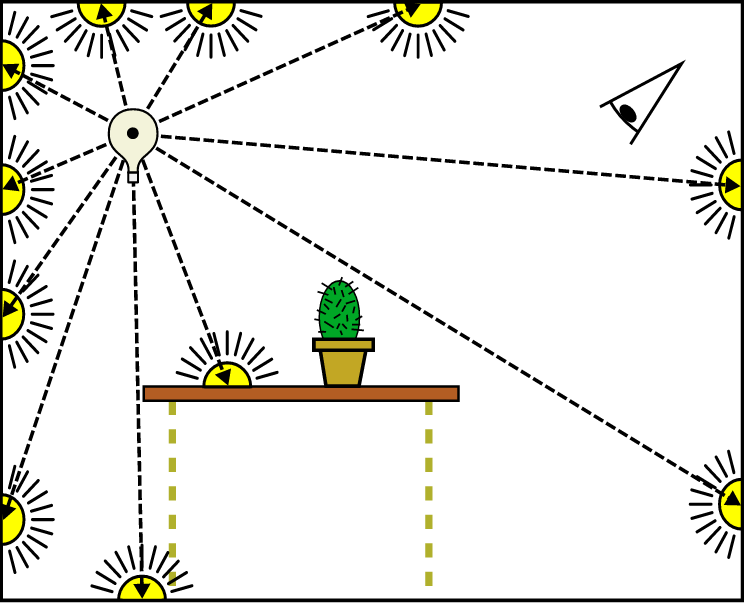
\includegraphics[width=.48\textwidth]{graphics/many_lights_laine_1} &
    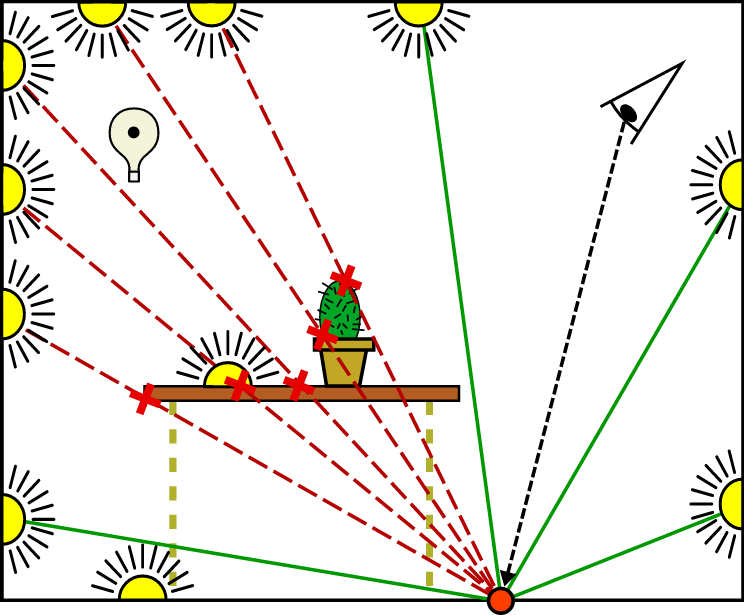
\includegraphics[width=.48\textwidth]{graphics/many_lights_laine_2}\\
  \end{tabular}
  \caption{Visualization of the many-light concept. (Left) VPLs are created on surfaces that are directly lit by a light source. (Right) when shading a surface point (orange), all VPLs that are visible for that point are used to indirectly light it. Figures reprinted from \citet{laine2007incremental}.}
  \label{fig:intro:many_lights_visualization}
\end{figure}

The use of many-light methods is intriguing since they are a natural and intuitive model of real-world light interactions. In addition the concept is highly scalable: Many-light methods have been used for real-time applications with up to a few thousand lights to offline rendering with millions of lights. Given enough lights, the concept is capable of accurately simulating advanced effects like subsurface scattering and participating media. Refer to \citet{Dachsbacher:2014:ManyLightsSTAR} for the higher-end spectrum of many-light methods.

Of course, when used for real-time applications the available performance budget enforces the use of a limited number of lights. With a few thousand lights at most, many effects are not possible to simulate anymore. Due to the low-frequency nature of diffuse reflections, however, several approximations can be made so that global illumination is still feasible to create with convincing results. In real-time applications, a different advantage comes into play: Since the method uses more or less conventional point light sources, many techniques from classical real-time rendering are applicable, such as point light rendering including conventional shadow maps for visibility testing. This makes basic implementations easy to create, even though more advanced techniques are necessary to achieve high performance.



\subsection{Components of Many-Light Methods}
This section will take the components of global illumination identified in \Cref{sec:intro:gi:components} and explain how they translate to many-light methods.

\paragraph{Direct lighting or light injection}
In theory, many-light methods do not need a light injection step since they are usually iterative processes that start with the scene lights and from there on, create new lights wherever the current light set lights the scene. In practice, the first bounce is often handled separately for performance reasons, and because the VPLs have different characteristics than most scene lights.

\paragraph{Light propagation}
As just mentioned, many-light methods can simulate an arbitrary number of light bounces by repeating the propagation step with an expanding set of VPLs. However, many techniques (and this thesis) simulate just the first bounce, since that alone provides a large quality enhancement over simulating no GI at all, and subsequent bounces are more complex in terms of implementation and computation.
\\
\\
Since the budget of VPLs is limited and it is thus desirable to get the maximum effect out of each VPL, much research has gone into efficient \textbf{VPL placement}. Both the light injection and light propagation step create VPLs and can take considerable amounts of computation time through complex sampling methods. Some techniques also do not distinguish between light injection and light propagation and have a unified process for placing VPLs.

\paragraph{Final gathering}
Most many-light methods perform final gathering per screen-space pixel. There are two main approaches commonly referred to as splatting and gathering. Both are too slow to use every light to shade every pixel, therefore optimizations and approximations are used. More on this in the next section.

\paragraph{Visibility testing}
Many-light methods provide no means of visibility computation; these need to be solved separately. The advantage of many-light methods is that each receiving element only needs to test the (bounded) number of VPLs for visibility, not an arbitrarily high number of scene elements. In contrast to other global illumination methods, this makes it possible (although not performant) to use shadow maps for visibility testing.

\paragraph{Choice of receiving elements}
As mentioned before, screen-space pixels are most commonly used, albeit often downscaled or combined with interleaved sampling (see \Cref{sec:intro:relatedWorkManyLight:finalGathering}). The other options listed in \Cref{sec:intro:gi:components} are technically possible as well, but haven't been combined with many-light methods yet.
\\
\\
Another challenge that is unique to many-light methods is \textbf{mitigating singularities}. Since the entire energy of the indirect light bounces is concentrated into a few infinitely small light sources, the areas near these light sources receive too much light. This effect is distinctly visible as bright spots around the VPL's location, making it necessary for many-light methods to alleviate this artifact.



\section{Previous Work on Real-Time Many-Light Methods}
\label{sec:intro:relatedWorkManyLight}

The following will present several many-light methods while concentrating on those that are applicable to real-time rendering. This section is structured roughly according to the different design decisions to be taken when applying many-light methods: VPL sampling, computing visibility, final gathering and mitigating singularities. The light transport step is not covered separately as it is often either omitted, simulating only one bounce, or integral part of the VPL sampling algorithm. The choice of receiving elements is not covered as well, as most papers in this area simply use screen-space pixels.

\citet{Dachsbacher:2014:ManyLightsSTAR} provide another overview over many-light methods, including those unsuitable for real-time rendering.


\subsection{Virtual Point Light Sampling}
\label{sec:intro:relatedWorkManyLight:vplSampling}

While \citet{Keller:1997:InstantRadiosity} uses an approach similar to photon mapping to create VPLs, real-time applications are in need of something more performant. A commonly used technique are \emph{reflective shadow maps} (RSMs, \cite{Dachsbacher:2005:RSM}), which use rasterization to create first-order VPLs. While in this paper, each pixel of the RSM is considered a VPL and during gathering, a random subset of all VPLs is sampled, beginning with \citet{dachsbacher2006splatting} most papers sample the RSM to create a fixed set of VPLs which is used during shading.

\citet{georgiev2010simple, ritschel2011ismsViewAdaptive} sample the RSM to create a set of VPLs with (estimated) high contributions to the final image. \citet{dong2009real, prutkin2012reflective} cluster several samples to form \emph{virtual area lights} (VALs). They observe that far fewer VALs than VPLs are necessary to achieve the same quality at a minor performance expense.

Most of these approaches suffer from poor temporal stability. To improve on that, \citet{laine2007incremental} update only a portion of the VPLs per frame but introduce latency to the indirect light, additionally dynamic objects can receive but not bounce light. \citet{barak2013temporally} provide temporally stable results with dynamic scene geometry, but not with moving light sources. \citet{hedman2016sequential} achieve near-optimal temporal stability even with moving light sources while maintaining high per-image accuracy at real-time frame rates. They use one classic shadow map per VPL though, which must be updated lazily to stay within real-time limits.


\subsection{Final Gathering}
\label{sec:intro:relatedWorkManyLight:finalGathering}

Splatting techniques have been used to add a light's contribution to the rendered image \citep{dachsbacher2006splatting, Nichols:2009:splatting}, but do not utilize modern GPUs efficiently. Instead, gathering approaches are commonly used today, using interleaved sampling \citep{Keller:2001:InterleavedSampling} to reduce the number of lights processed per pixel, in combination with an edge-aware blur similar to \citet{laine2007incremental}. \citet{segovia2006non} improve the cache efficiency of interleaved sampling.


\subsection{Visibility Computation}
\label{sec:intro:relatedWorkManyLight:visibility}

Several approaches exist to calculate visibility between VPLs and the scene parts visible to the camera. Classic shadow maps are a fairly exact solution, but cannot be updated every frame for the several hundreds or even thousands of VPLs.

A popular approach are \emph{imperfect shadow maps} \citep[ISMs,][]{ritschel2008ism}, which use a precomputed set of points as scene representation to quickly render large amounts of small and inaccurate shadow maps. \citet{ritschel2011ismsViewAdaptive} extend the approach to fully dynamic scenes among other improvements. \citet{barak2013temporally} use tessellation to compute the point set, eliminating the need to keep a separate point set updated, making it inherently dynamic and providing better performance for larger point sets.

Ray-tracing has been proposed to compute visibility as well \citep[e.\,g.][]{segovia2006bidirectional}, but suffers from the usual drawbacks of ray-tracing in a real-time context. A voxel-based scene representation has also been used to perform visibility queries for many-light techniques \citep{sun2015manylightsSVO}.


\subsection{Mitigating Singularities}
\label{sec:intro:relatedWorkManyLight:singularities}

In naive implementations of many-lights techniques, bright spots will appear near the VPL’s positions due to the light’s attenuation term approaching infinity. A common approach is to clamp the term. This introduces bias, which can be compensated e.\,g.\ in screen space \citep{novak2011screen}. Singularities can also be avoided through more advanced light representations \citep{tokuyoshi2015vsgl}.


\cleardoublepage
